\documentclass[12pt,english]{article}

\usepackage{amsmath,amssymb,amsthm,epsfig,lineno,rotfloat,psfrag,natbib,caption,setspace,url,bm,geometry}
\usepackage{ecology}
\usepackage{graphicx}

\geometry{verbose,letterpaper,tmargin=2.54cm,bmargin=2.54cm,lmargin=2.54cm,rmargin=2.54cm}

%\setlength{\evensidemargin}{0in} \setlength{\oddsidemargin}{0in}
%\setlength{\topmargin}{-0.65in} \setlength{\textwidth}{6.5in}
%\setlength{\textheight}{9.5in} \setlength{\topskip}{0in}
%\setlength{\headheight}{0in}


%\newcommand{\yst}{\ensuremath{y_{st}}}
%\newcommand{\tyst}{\ensuremath{\tilde y_{st}}}
%\newcommand{\tzs}{\ensuremath{\tilde z_{s}}}
%\newcommand{\zs}{\ensuremath{z_{s}}}
%\newcommand{\bg}{\ensuremath{\boldsymbol{\gamma}}}
%\newcommand{\bxs}{\ensuremath{\mathbf{x}_{s}}}
%\newcommand{\bxst}{\ensuremath{\mathbf{x}_{st}}}
%\newcommand{\bK}{\ensuremath{\mathbf{K}}}
%\newcommand{\bn}{\ensuremath{\boldsymbol{\eta}}}
%\newcommand{\bb}{\ensuremath{\boldsymbol{\beta}}}
%\newcommand{\ba}{\ensuremath{\boldsymbol{\alpha}}}
%\newcommand{\by}{\ensuremath{\mathbf{y}}}
%\newcommand{\bz}{\ensuremath{\mathbf{z}}}
%\newcommand{\bX}{\ensuremath{\mathbf{X}}}
%\newcommand{\be}{\ensuremath{\boldsymbol{\epsilon}}}
%\newcommand{\bQ}{\ensuremath{\mathbf{Q}}}
%\newcommand{\bO}{\ensuremath{\boldsymbol{\Omega}}}
%\newcommand{\bm}{\ensuremath{\boldsymbol{\mu}}}






\bibliographystyle{ecology}
\raggedbottom


\captionsetup[table]{margin=0pt,font=small,labelfont={sc},justification=justified,labelsep=period}
\captionsetup[figure]{margin=0pt,font=small,labelfont={sc},justification=justified,labelsep=period,name=Fig}



\begin{document}
\begin{spacing}{1.9}

\begin{center}
Avoiding extrapolation bias when using statistical models to make ecological prediction
\bigskip\\
\normalsize
{\sc Paul B. Conn$^{1,}$\footnotemark[2] and
Devin S. Johnson$^1$, Peter L. Boveng$^1$ }\smallskip\\
$^1${\em National Marine Mammal Laboratory, NOAA, National Marine Fisheries Service,
Alaska Fisheries Science Center, 7600 Sand Point Way NE, Seattle,
WA 98115 USA }\\ \medskip
\end{center}
\footnotetext[2]{Email: paul.conn@noaa.gov}


\raggedright \setlength{\parindent}{0.3in}
%\renewcommand{\baselinestretch}{1.8}\normalsize
\clubpenalty=0
 \linenumbers


{\em Abstract.\ } We'll do this later



{\em Key words: Abundance, Extrapolation, General additive models, Generalized linear models, Independent Variable Hull, Leverage, Prediction variance, Spatial regression, Species distribution model}

\centerline{\sc Introduction}


In ecology and conservation, a common goal is to make predictions about an unsampled random variable given a limited sample from the target population.  For instance, given a model ($\mathcal{M}$), estimated parameters ($\hat{\boldsymbol{\theta}}$), and a covariate vector ${\bf x}_i$, we often desire to predict a new observation $y_{new}$ at $i$.  For instance, we might use a generalized linear model \citep{McCullaghNelder1989} or one of its extensions to predict species density or occurrence in a new location, or to predict the future trend of a population.

Early in their training, ecologists and statisticians are warned against extrapolating statistical relationships
past the range of observed data.  This caution is easily interpreted in the context of single-variable linear regression analysis; one should be cautious in using the fitted relationship to make predictions at some new point $y_{new}$ whenever $x_{new} < \min({\bf x})$ or $x_{new} > \max({\bf x})$.  But what about more complicated situations
where there are multiple explanatory variables, or when one uses a spatial regression model to account for the residual spatial autocorrelation that is inevitably present in patchy ecological data \citep{LichsteinEtAl2002}?  How reliable are spatially- or temporally-explicit predictions in sophisticated models for animal abundance and occurrence?

Statisticians have long struggled with the conditions under which fitted regression models are capable of
making robust predictions at new combinations of explanatory variables.  The issue is sometimes considered more of a
philosophical problem than a statistical one, and has even been likened to soothsaying \citep{EhrenbergBound1993}.  To our mind, the reliability of predictions from statistical models is likely a function of several factors, including (i) the intensity of sampling,
(ii) spatial or temporal proximity of the prediction location to locations where there are data, (iii) variability of the ecological process, and (iv) the similarity of explanatory covariates in prediction locations when compared to the ensemble of covariates for observed data locations.

Our aim in this paper is to investigate extrapolation bias in the generalized linear model and its extensions, including generalized additive models \citep[GAMs;][]{HastieTibshirani1999,Wood2006} and spatial, temporal, or spatio-temporal regression models (STRMs).  In particular, we exploit some of the same ideas used in multiple linear regression regarding leverage and outliers \citep{Cook1979} to operationally define ``extrapolation" as making predictions that occur outside of a generalized independent variable hull (gIVH) of observed data points. Application of the gIVH and related criterion (e.g. prediction variance) can provide intuition regarding the reliability of predictions in unobserved locations, and can aid in model construction.  Also, since the gIVH can be constructed solely with knowledge of sampled locations and explanatory covariates (i.e., it does not necessarily require any observed response variables), it can also be used to help guide survey design. We illustrate use of the gIVH on a simulated occupancy dataset, on a species distribution model (SDM) for ribbon seals in the eastern Bering Sea, and on a population trend model for Steller Sea Lions ({\it Phoca fasciata}).

\section{The generalized independent variable hull (gIVH)}

Extrapolation is often distinguished from interpolation.  In a prediction context, we might define (admittedly quite imprecisely) that extrapolation consists of making predictions that are ``outside the range of observed data" while interpolation consists of making predictions ``inside the range of observed data."  But what exactly do we mean by ``outside the range of observed data"?  Predictions outside the range of observed covariates?  Predictions for locations that are so far from places where data are gathered that we are skeptical that the estimated statistical relationship still holds? To help guide our choice of an operational definition, we turn to early work on outlier detection in simple linear regression analysis.

In the context of outlier detection, Cook (\citeyear{Cook1979}) defined an independent variable hull (IVH) as the smallest convex set containing all design points of a full-rank linear regression model.  Linear regression models are often written in matrix form, i.e.
\begin{linenomath*}
\begin{equation*}
  {\bf Y} = {\bf X} \boldsymbol{\beta} + \boldsymbol{\epsilon},
\end{equation*}
\end{linenomath*}
where ${\bf Y}$ give observed data, ${\bf X}$ is a so-called design matrix that includes explanatory variables \citep[see e.g.][]{Draper1966}, and $\boldsymbol{\epsilon}$ represent normally distributed residuals (here and throughout the paper, bold symbols will be used to denote vectors and matrices).
Under this formulation, the IVH is defined relative to the hat matrix, ${\bf V}_{\rm LR}={\bf X}({\bf X}^\prime{\bf X})^{-1}{\bf X}^\prime$ (where the subscript ``LR" denotes linear regression).  Letting $v$ denote the maximum diagonal element of ${\bf V}_{LR}$, one can examine whether a new design point, ${\bf x}_0$ is within the IVH.  In particular, ${\bf x}_0$ is within the IVH whenever
\begin{linenomath*}
\begin{equation}
  \label{eq:IVH}
  {\bf x}_0^\prime ({\bf X}^\prime{\bf X})^{-1}{\bf x}_0 \le v.
\end{equation}
\end{linenomath*}
Cook (\citeyear{Cook1979}) used this concept to identify influential observations and possible outliers, arguing that design points near the edge of the IVH are deserving of special attention.  Similarly, points outside the IVH should be interpreted with caution.

We simulated two sets of design data to help illustrate application of the IVH (Fig. \ref{fig:IVH}).  In simple linear regression with one predictor variable, predictions on a hypothetical response variable obtained at covariate values below the lowest observed value or above the highest observed value are primarily outside of the IVH.  We suspect this result conforms to most ecologists intuition about what constitutes ``extrapolating past the observed data."  However, fitting a quadratic model exhibits more nuance; if there is a large gap between design points, it is entirely possible that intermediate covariate values will also be outside of the IVH and thus more likely to result in problematic predictions.  Fitting a model with two covariates and both linear and quadratic effects, the shape of the IVH is somewhat more irregular, and even includes a hole in the middle of the surface when interactions are modeled (Fig. \ref{fig:IVH}).  These simple examples highlight the sometimes counterintuitive nature of the predictive inference problem, a problem that can only become worse as models with more dimensions are contemplated (including those with temporal or spatial structure).  Fortunately, the ideas behind the IVH provide a potential way forward.

Cook's (1979) formulation for the IVH is particular to linear regression analysis, which assumes iid Gaussian error. Thus, it is not directly applicable to generalized models, such as those including alternative error distributions (e.g., Poisson, binomial) or spatial random effects.  Further, the hat matrix is not necessarily well defined for models with more general spatial structure. However, since the hat matrix is proportional to prediction variance, Cook (1979) notes that design points with maximum prediction variance will be located on the boundary of the IVH.  We therefore define a generalized independent variable hull (gIVH) as the set of all points ${\bf x}$ (note that ${\bf x}$ can include both observed and unobserved design points) such that
\begin{linenomath*}
\begin{equation}
  \label{eq:gIVH}
  {\rm var}({\bf y}_x | {\bf x}) \le {\rm max} [{\rm var}({\bf y}_X | {\bf X})],
\end{equation}
\end{linenomath*}
where ${\bf Y}_x$ correspond to predictions at ${\bf x}$, and ${\bf X}$ and ${\bf Y}_X$ denote observed design points and predictions at $X$, respectively.

Generalizations of the linear model are often written in the form
\begin{linenomath*}
\begin{equation}
  Y_i \sim f_Y(g(\mu_i)),
\end{equation}
\end{linenomath*}
where $f_Y$ denotes a probability density or mass function (e.g. Bernoulli, Poisson), $g$ gives an inverse link function, and
$\mu_i$ is a predictor.  For many such generalizations, it is possible to specify the $\mu_i$ as
\begin{linenomath*}
\begin{equation}
  \boldsymbol{\mu} = {\bf X}_{aug}\boldsymbol{\beta}_{aug} + \boldsymbol{\epsilon},
  \label{eq:mu-aug}
\end{equation}
\end{linenomath*}
where the $\boldsymbol{\epsilon}$ represent Gaussian error, ${\bf X}_{aug}$ denotes an augmented design matrix, and $\boldsymbol{\beta}_{aug}$ denote an augmented vector of parameters.  For instance, in a spatial model, $\boldsymbol{\beta}_{aug}$ might include both fixed effect parameters and spatial random effects in a reduced dimension subspace (see Appendix A for examples of how numerous types of models can be written in this form).

When models are specified as in Eq. \ref{eq:mu-aug}, we can write prediction variance generically as
\begin{linenomath*}
\begin{equation}
  \label{eq:var-mu}
  {\rm var}(\boldsymbol{\mu}_x | {\bf x})= {\bf x} {\rm var}(\hat{\boldsymbol{\beta}}_{aug}) {\bf x}^\prime,
\end{equation}
\end{linenomath*}
where it is understood that the exact form of ${\bf x}$ and ${\rm var}(\hat{\boldsymbol{\beta}}_{aug})$ depends on the model chosen (i.e., GLM, GAM, or STRM; Appendix A). This expression for prediction variance is on the linear predictor scale; if a non-identity link function is used, we can use the delta method \citep{Dorfman1938,VerHoef2012} to approximate prediction variance on the real scale (i.e. the scale in which data are measured) as
\begin{linenomath*}
\begin{eqnarray*}
  \label{eq:var-mu}
  {\rm var}(g(\mu_x) | {\bf x}) & = & \boldsymbol{\Delta} {\rm var}(\boldsymbol{\mu}_x | {\bf x})\boldsymbol{\Delta}^\prime, 
%  \boldsymbol{\Delta} & = & \left[ \begin{array}{cccc}
%      \frac{\partial g(\mu_1)}{\partial \mu_1} & \frac{\partial g(\mu_1)}{\partial \mu_2} & %\hdots & \frac{\partial g(\mu_1)}{\partial \mu_n} \\
%      \frac{\partial g(\mu_2)}{\partial \mu_1} & \frac{\partial g(\mu_2)}{\partial \mu_2} & %\hdots & \frac{\partial g(\mu_2)}{\partial \mu_n} \\
%      \vdots & \vdots & \ddots & \vdots \\
%      \frac{\partial g(\mu_n)}{\partial \mu_1} & \frac{\partial g(\mu_n)}{\partial \mu_2} & %\hdots & \frac{\partial g(\mu_n)}{\partial \mu_n} \\
%  \end{array} \right].
\end{eqnarray*}
\end{linenomath*}
where $\boldsymbol{\Delta}$ is a matrix of partial derivatives $\partial g(\mu_r)/\partial \mu_c$ ($r$ and $c$ denoting rows and columns of $\boldsymbol{\Delta}$, respectively).  Under common univariate link functions (e.g. log, logit, probit), $\boldsymbol{\Delta}$ has a diagonal form, while for multivariate links (e.g. multinomial logit) $\boldsymbol{\Delta}$ will be dense.

%For GLMs, prediction variance is proportional to the original hat matrix ${\bf V}_{LR}$ (at %least on the linear predictor scale), and Eq. \ref{eq:IVH} may be used directly.  For other %models, we have
%\begin{linenomath*}
%\begin{equation}
%  \label{eq:var_Beta}
%  {\rm var}(\hat{\boldsymbol{\beta}}_{aug})=\left[ \begin{array}{cc}
%      \boldsymbol{\Sigma}_\beta & {\bf 0}\\
%      {\bf 0} & \boldsymbol{\Sigma}_\alpha
%  \end{array} \right],
%\end{equation}
%\end{linenomath*}
%where we simply replace $\boldsymbol{\beta}_{aug}$ with the augmented vector that includes %both regression and spatial or smooth parameters (i.e. $\boldsymbol{\beta}$ and %$\boldsymbol{\alpha}$; Appendix S1).

The exact form of ${\rm var}(\hat{\boldsymbol{\beta}}_{aug})$ differs depending on the underlying model structure and estimation procedure.  In the following treatment, we shall focus on Bayesian analysis; although it is not necessarily needed to fit GLMs and GAMs, it helps make STRMs more computationally tractable and puts all of the different models into a common analysis framework.  This approach requires specifying priors for model parameters, and prior parameters may appear in expressions for prediction variance.  Judicious choices of priors can at times limit the influence of priors on calculation of the gIVH.  For example, if we specify the prior on the vector of regression coefficients to be $[\boldsymbol{\beta}] = \textrm{MVN}({\bf 0},(\tau_\beta X^\prime X)^{-1})$ where $\tau_\beta$ is a fixed constant, a Bayesian implementation of a GLM still results in the gIVH specified in Eq. \ref{eq:IVH}.  The ability to use Eq. 5 directly is quite useful, as we only need to know the explanatory variables to be able to diagnose whether predictions lie in or out of the gIVH. However, the other models considered here (GAMs and STRMs) typically require estimation of one or more precision or autocorrelation parameters.   In these cases, one solution is to impose prior distributions and integrate over these additional parameters (call them $\boldsymbol{\theta}$) to obtain an expectation for ${\rm var}(\hat{\boldsymbol{\beta}}_{aug})$.  Using the law of the unconscious statistician, we have
\begin{linenomath*}
\begin{equation}
  \label{eq:E_var_Beta}
  {\rm E}({\rm var}(\hat{\boldsymbol{\beta}}_{aug}))  = \int_{\boldsymbol{\theta}} {\rm var}(\hat{\boldsymbol{\beta}}_{aug}|\boldsymbol{\theta}) [\boldsymbol{\theta}] d \boldsymbol{\theta}.
\end{equation}
\end{linenomath*}
Here, and throughout the paper, we use the bracket notation to indicate a probability density function; e.g., $[\boldsymbol{\theta}] $ denotes the joint prior distribution for $\boldsymbol{\theta}$. If observations have already been gathered, one could also consider integrating over the marginal posterior distribution using MCMC:
\begin{linenomath*}
\begin{equation}
  \label{eq:E_var_Beta_post}
  {\rm E}({\rm var}(\hat{\boldsymbol{\beta}}_{aug}) | {\bf Y})  = \int_{\boldsymbol{\theta}} {\rm var}(\hat{\boldsymbol{\beta}}_{aug}|\boldsymbol{\theta}) [\boldsymbol{\theta}| {\bf Y}] d \boldsymbol{\theta}.
\end{equation}
\end{linenomath*}
Some care must be taken with prior distributions if Eq. \ref{eq:E_var_Beta} is used for calculation of prediction variance.  For instance, standard ``non-informative" or ``flat" priors may place substantial mass on implausible values.  When using the gIVH or prediction variance to help guide sampling design \citep[see][for an example using prediction variance]{DiggleLophaven2006}, we suggest using informative prior distributions.

We propose to use the gIVH in much the same manner as Cook (1979).  In particular, we use the gIVH to differentiate whether spatial predictions are interpolations (predictive design points lying inside the gIVH) or extrapolations (predictive design points lying outside the gIVH).  The gIVH, together with prior-integrated prediction variance, seem ideally situated to diagnosing potential extrapolation issues as it does not necessarily need to rely on gathered response data. Thus, one can examine whether or not prediction points lie within the gIVH without ever collecting response data there.  Further, one can compare prediction variance in places one has data to places where predictions are desired to gauge the relative amount of information that predictions are being based on.

\section{Examples}

\subsection{Simulation study}

We conducted a simulation study to investigate whether the gIVH (and accompanying prediction variance) was useful in diagnosing prediction biases when analyzing animal count data. For each of 100 simulations, we generated animal abundance over a $30 \times 30$ grid assuming that animal density was homogeneous in each grid cell.  Animal abundance was generated as a function of four hypothetical habitat covariates (Appendix B).   For each simulated landscape, we randomly selected 60 grid cells for sampling, assuming that sampling quadrats encompassed 10\% of the area of each selected grid cell.  For ease of presentation and analysis, we assumed detection probability was 100\% in each quadrat.  Once animal counts were simulated, three different estimation models were fitted to the data: a GLM, a GAM, and an STRM (Appendix B).  The GLM and STRM expressed log-density as a function of linear and quadratic covariate effects, while the GAM used a kernel smoother with 4 knots for each covariate (Appendix B).  Each model was provided with three of the four covariates used to generate the data.

For each simulated data set and model structure, we calculated (1) $\text{gIVH}_{int}$, the gIVH resulting from integrating over prior parameter variance (i.e. using Eq. \ref{eq:E_var_Beta} with informative priors), and (2) $\text{gIVH}_{post}$, the gIVH arising from posterior predictive variance (i.e. posterior variance when data are actually analyzed).  We then calculated posterior predictions of animal abundance within and outside of each gIVH in order to gauge bias as a function of whether or not inference is constrained to the gIVH.  Specifically, the performance of the $\text{gIVH}_{int}$ criterion in diagnosing extrapolation bias is a test of whether it is useful in designing animal count surveys, while the performance of $\text{gIVH}_{post}$ may help decide its utility in limiting the scope of landscape-based inference once data have been collected and analyzed.





\subsection{Ribbon seal SDM}
As part of an international effort, researchers with the U.S. National Marine Fisheries Service conducted aerial surveys over the eastern Bering Sea in 2012 and 2013.  Agency scientists used infrared video to detect seals that were on ice, and simultaneous automated digital photographs provided information on species identity. Here, we use spatially referenced count data from photographed ribbon seals, {\it Phoca fasciata} (Fig. \ref{fig:ribbon}) on a subset of 10 flights flown over the Bering Sea in April 2012.  These flights were limited to a one week period so that both sea ice conditions and seal distributions could be assumed to be static.

Our objective with this dataset will be to model seal counts on transects through 25km by 25km grid cells as a function of habitat covariates and possible spatial autocorrelation. Estimates of apparent abundance can then be obtained by summing predictions across grid cells. Figure \ref{fig:flights} shows the transects flown and the number of ribbon seals encountered in each cell, and Figure \ref{fig:covs} show explanatory covariates gathered to help predict ribbon seal abundance.  These data are described in fuller detail by \citet{ConnEtAl2014}, who extend the modeling framework of STRMs to account for incomplete detection and species misidentification errors \citep[see e.g.][]{ConnEtAl2014}.  Since our focus in this paper is on illustrating spatial modeling concepts, we devote our efforts to the comparably easier problem of estimating apparent abundance (i.e., uncorrected for vagaries of the detection process).

Inspection of ribbon seal data (Fig. \ref{fig:flights}) immediately reveals a potential
issue with spatial prediction: abundance of ribbon seals appears to be maximized in the southern and/or southeast quadrant of the surveyed area.  Predicting abundance in areas further south and east may thus prove problematic.  To illustrate, let $Y_i$ denote the ribbon seal count ($Y_i$) obtained in sampled grid cell $i$.  Suppose that counts arise according to a log-Gaussian Cox process, such that
\begin{eqnarray}
  \label{eqn:Cox}
  Y_i \sim {\rm Poisson}(\lambda_i) \mbox{ and } \\
  \log(\lambda_i) = \log(P_i) + {\bf X}_i \boldsymbol{\beta} + \eta_i + \epsilon_i, \nonumber
\end{eqnarray}
where $P_i$ gives the proportion of area photographed in grid cell $i$ (recall also that ${\bf X}_i$ denotes a vector covariates for cell $i$, $\boldsymbol{\beta}$ are regression coefficients, $\eta_i$ represents a spatially autocorrelated random effect, and $\epsilon_i$ is normally distributed $iid$ error).

We could fit any number of predictive models to these data, but we start with a simple
generalized linear model where we ignore the spatial random effect, $\eta_i$, and use the full suite of predictor covariates (Fig. \ref{fig:covs}) to fit Eq. \ref{eqn:Cox} to our data. In particular, we fit a model with linear effects of all predictor variables, and with an additional quadratic term for ice concentration \citep[seal density is often maximized at an intermediate value of ice concentration; see][]{VerHoef2013,ConnEtAl2014}. To enable comparison with more complicated types of models, we formulated a generalized Bayesian strategy for parameter estimation (see Appendix S1).  For simplicity, we generated posterior predictions of ribbon seal abundance across the landscape as
\begin{equation}
  N_i \sim {\rm Poisson}(A_i \lambda_i),
\end{equation}
where $A_i$ gives the proportion of suitable habitat in cell $i$ (ribbon seals do not inhabit land masses).

Fitting this model to our data,





\subsection{Steller sea lion trends}




\section{Discussion}

A number of authors have explored optimal knot placement in spatial models.  In the context of predictive process modeling \citep[where a covariance function is specified over a group of knots; see][]{BanerjeeEtAl2008}, \citet{FinleyEtAl2009} and \citet{GelfandEtAl2013} considered near-optimal knot placement by minimizing spatially averaged prediction variance.
Gelfand et al. knot selection

Using GAs to select knot placement using


Contrast with posterior loss (e.g., Jay's linex loss function estimator)

Contrast with cross validation

David Miller (the evil one)/Simon Wood stuff on edge effects

Contrast with other approaches-
Gelfand et al. Bayesian analysis - intrinsic CAR in SDM
Chakraborty et al. '10 - spatial abundance modeling - ordinal
Latimer et al. 2009 - spatial predictive process modelling in SPDs

Can't be complacent... still possible to get poor/biased results, e.g. if $\tau_\epsilon \rightarrow 0$.  Can't resolve pathological problems.

Presence-absence data, other link functions (e.g. probit)

extensions to models w/ secondary observation process, measurement error

much attention has been given to collinearity in multiple linear regression - suggest researchers give as much attention to predictive extrapolation bias in predictive models

For predictions with spatial , our experience is that predictions outside the minimum convex polygon where data are obtained can sometimes be more problematic than predictions within the polygon.  Spatial prediction surfaces may have a tendency to bend up or down in these areas, resulting in ``edge effects" that can lead to positive prediction bias when a log link function is employed \citep{VerHoefJansen2007}.

Fieberg PVA

\bibliography{master_bib}


FIGURE 1. A ribbon seal, {\it Phoca fasciata}; the focus of spatial modeling efforts in this paper.

FIGURE 2. Examples IVHs constructed from simulated data.  In panels A and B, the investigator plans to model a hypothetical (unmeasured) response variable using a linear regression model as a function of a single covariate, $x$, obtained at a number of design points (denoted with an ``x").  Using $x$ as a simple linear effect (A), only predictions less than the minimum observed value of $x$ or greater than the maximum value of $x$ are outside the IVH (shaded area), as scaled prediction variance in these areas (solid line) are greater than the maximum scaled prediction variance for observed data (dashed line).  Using both linear and quadratic effects of $x$, some intermediate points are also outside the IVH; predictions at these points should also be viewed with some caution.  Panels C $\&$ D show a more complicated IVH when the investigator wishes to relate an unmeasured response variable to linear and quadratic effects of two covariates, $x$ and $y$, either without interactions (C) or with interactions (D).  Any potential predictions in the shaded area are outside of the IVH.

FIGURE 3. Aerial surveys over the Bering Sea in spring of 2012 (blue lines) overlayed on
a tesselated surface composed of 25km by 25km grid cells.  Gray indicates land, and colored pixels indicate ribbon seal encounters (yellow: 1-2 seals; orange: 3-4 seals; magenta: 5-9 seals; red: 10-15 seals).  On average, photographs covered approximately $2.6km^2$ ($0.4\%$) of each surveyed grid cell.

FIGURE 4. Potential covariates gathered to help explain and predict ribbon seal abundance in the eastern Bering Sea.  Covariates include distance from mainland (\texttt{dist\_mainland}), distance from 1000m depth contour (\texttt{dist\_shelf}), average remotely sensed sea ice concentration while surveys were being conducted (\texttt{ice\_conc}), and distance from the southern sea ice edge (\texttt{dist\_edge}).  All covariates except ice concentration were standardized to have a mean of 1.0 prior to plotting and analysis.

FIGURE 5  Posterior median estimates of ribbon seal apparent abundance across the eastern Bering sea for (A) a generalized linear model (GLM), (B) a generalized additive model (GAM), (C) a GLM with known zero data, and (D) a GAM with known zero data.  Highlighted cells indicate those where predictive covariate values are outside of the generalized independent variable hull.

\clearpage
\centerline{\sc Figures}



\begin{figure}[!h]
\begin{center}
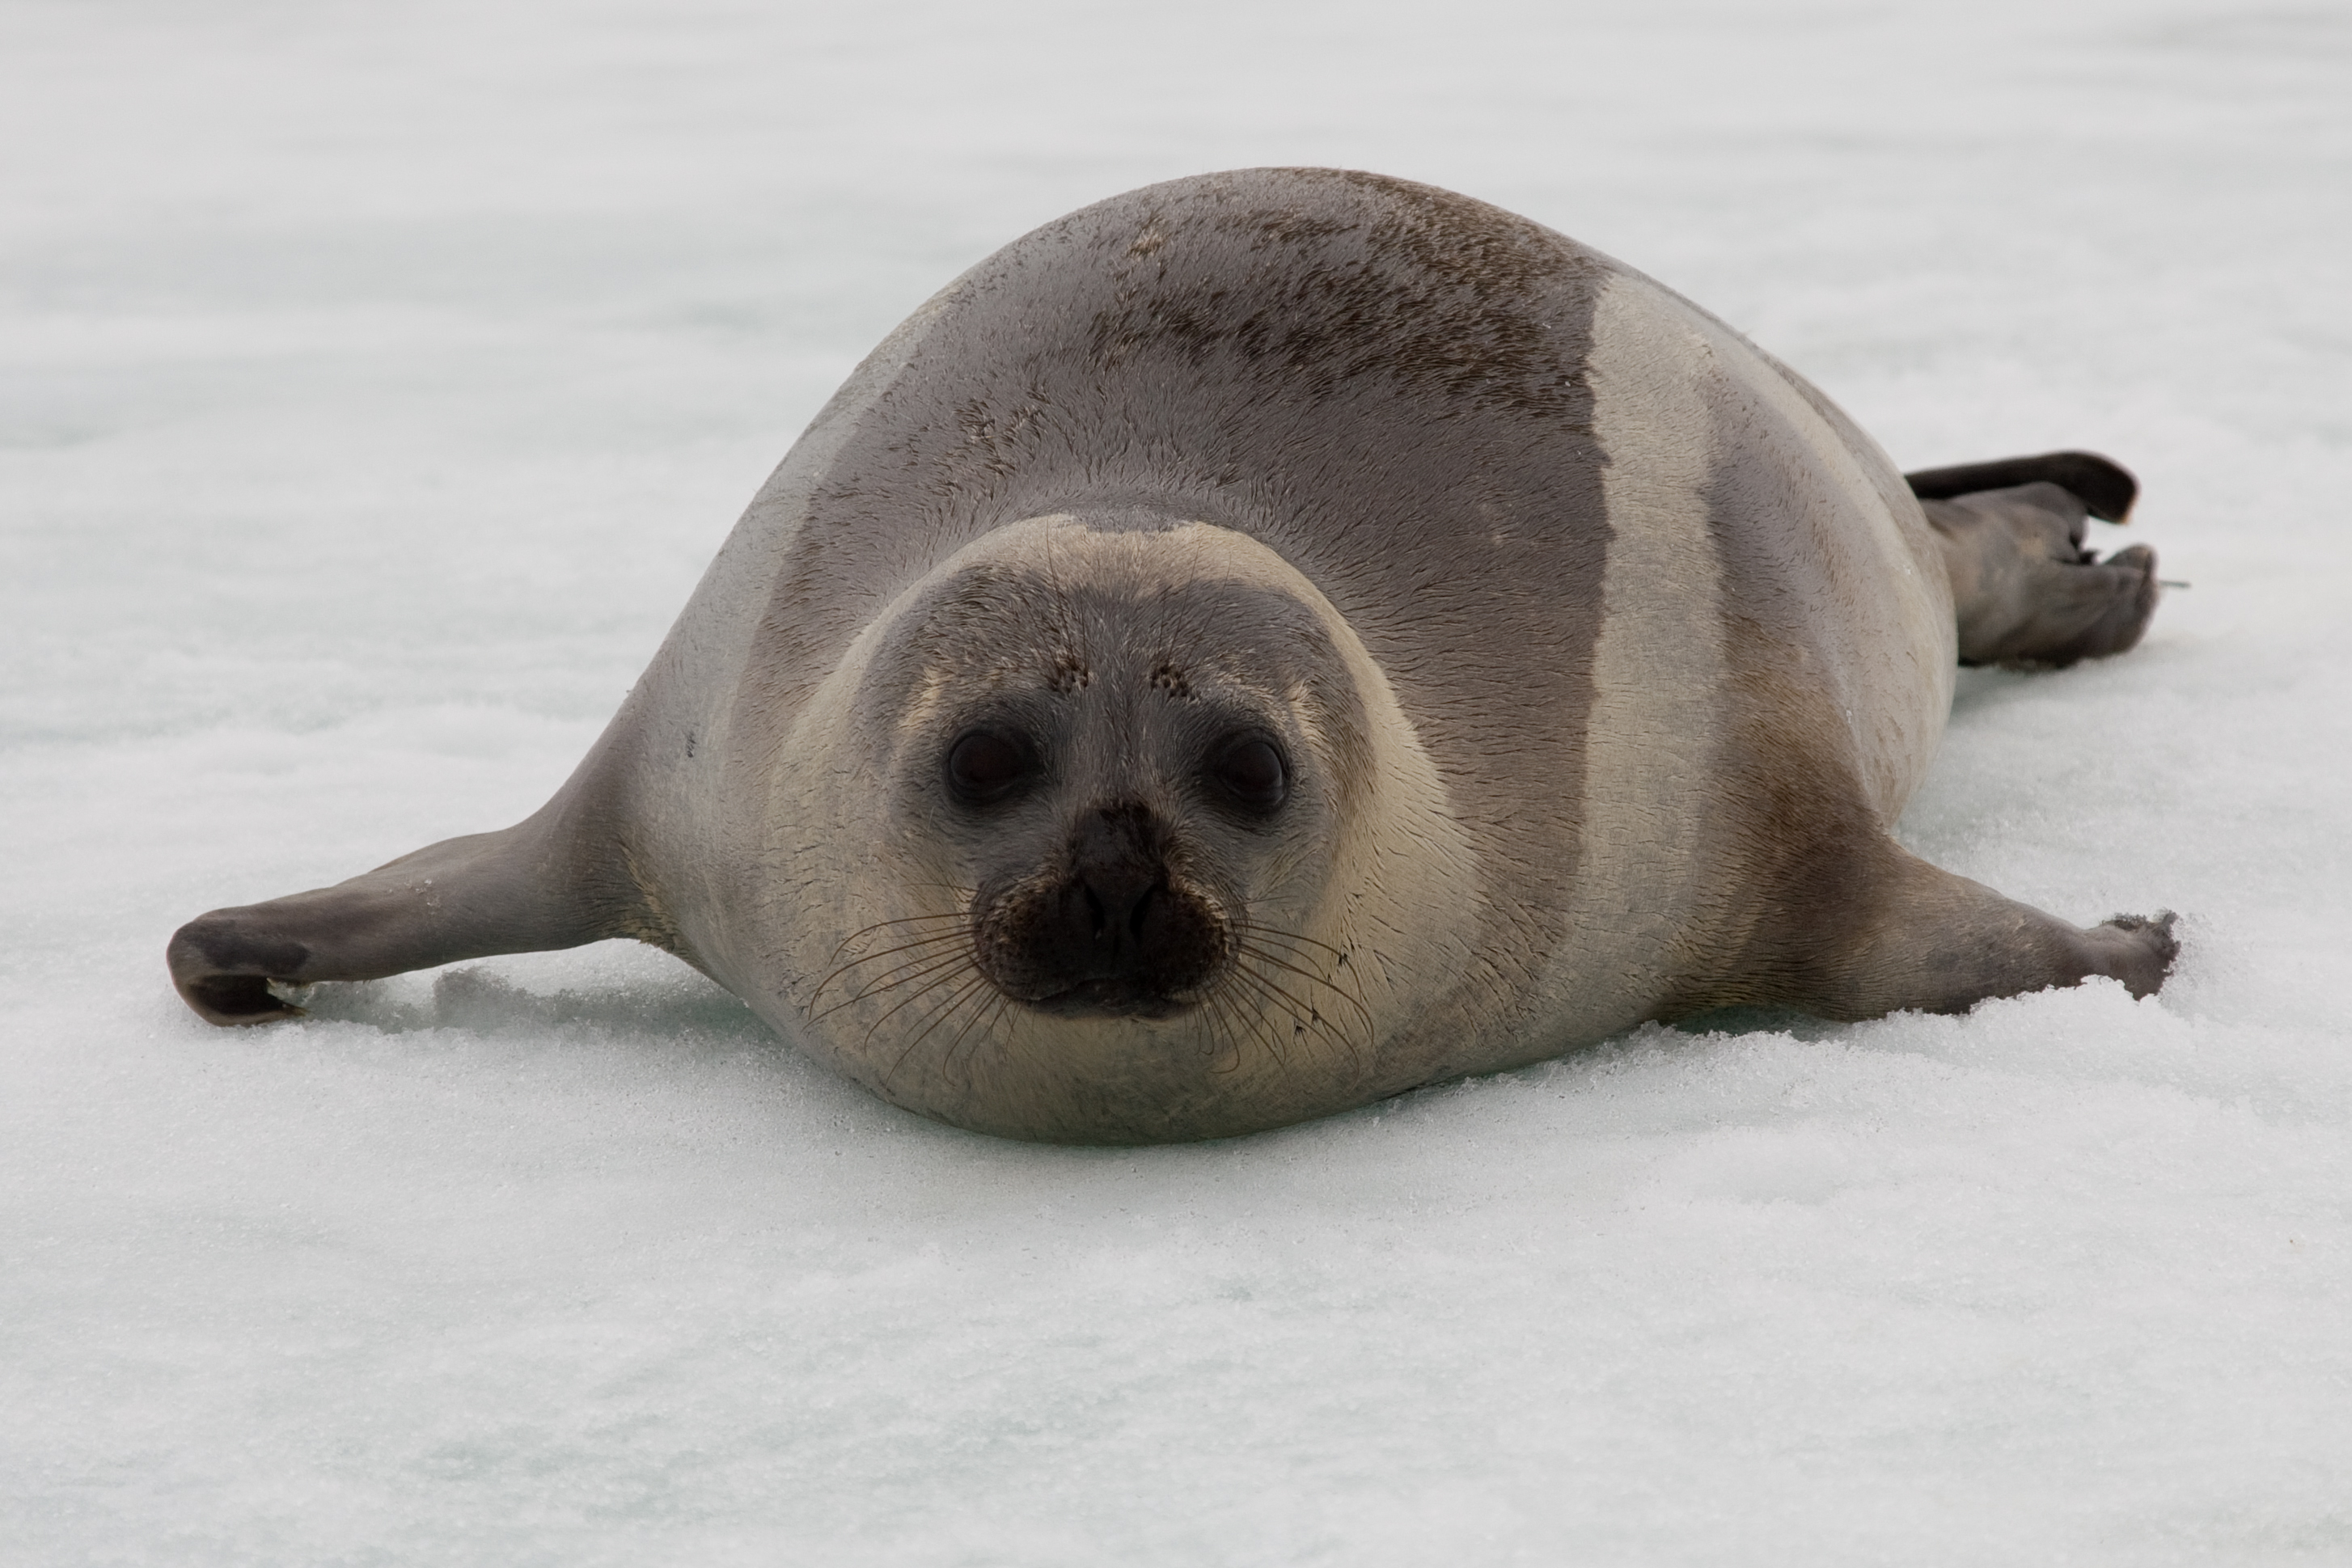
\includegraphics[width=6in]{ribbon}
\end{center}
\caption{ }
\label{fig:ribbon}
\end{figure}

\begin{figure}[!h]
\begin{center}
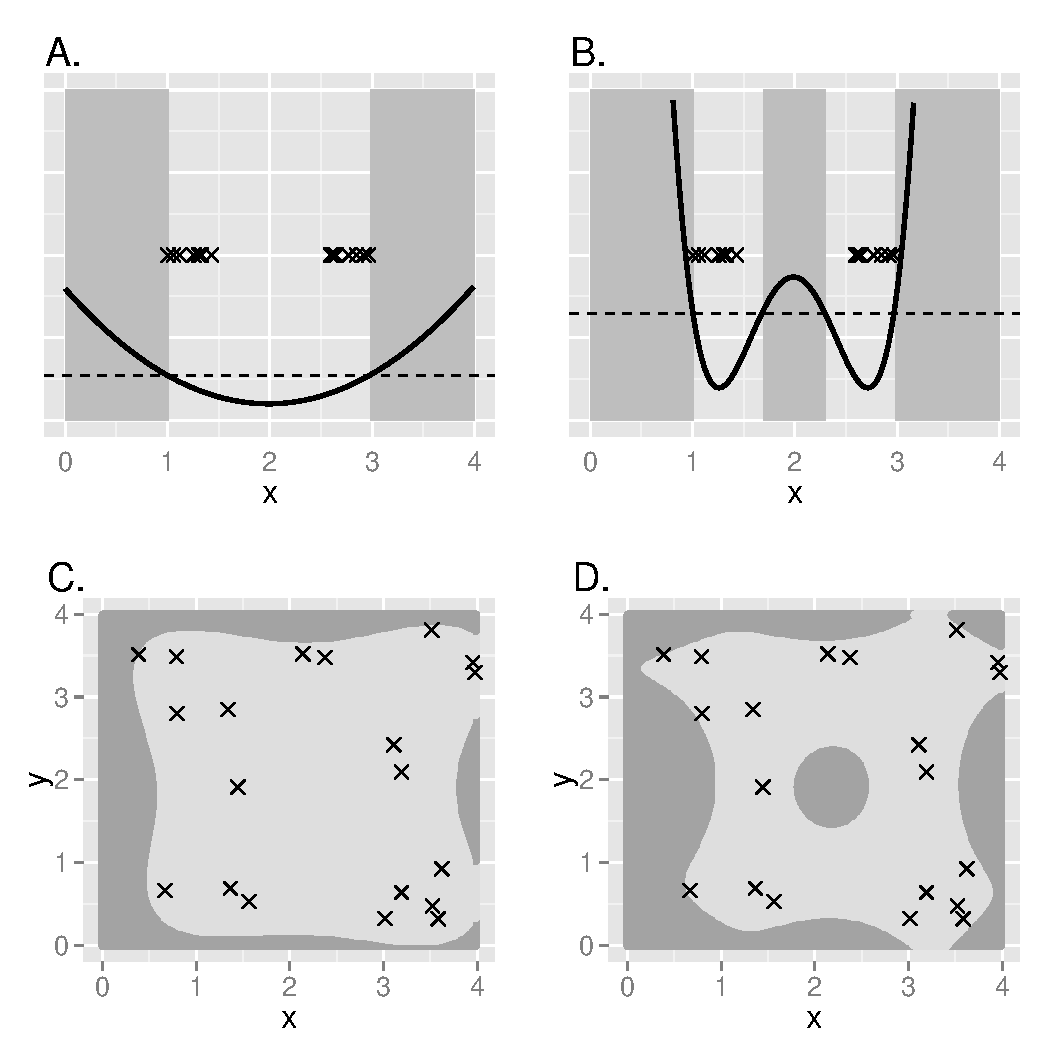
\includegraphics[width=6in]{IVH_simple2.pdf}
\end{center}
\caption{ }
\label{fig:IVH}
\end{figure}

\begin{figure}[!h]
\begin{center}
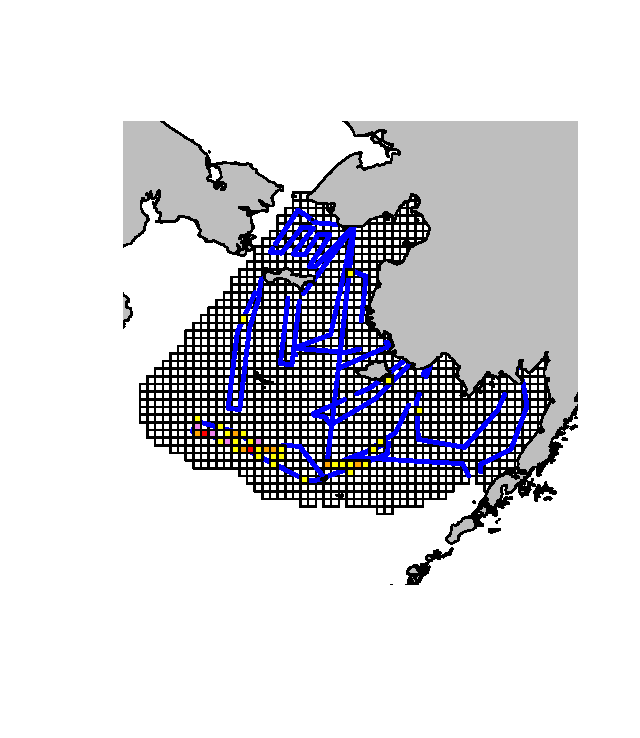
\includegraphics[width=6in]{test_flights_optimized.pdf}
\end{center}
\caption{ }
\label{fig:flights}
\end{figure}

\begin{figure}[!h]
\begin{center}
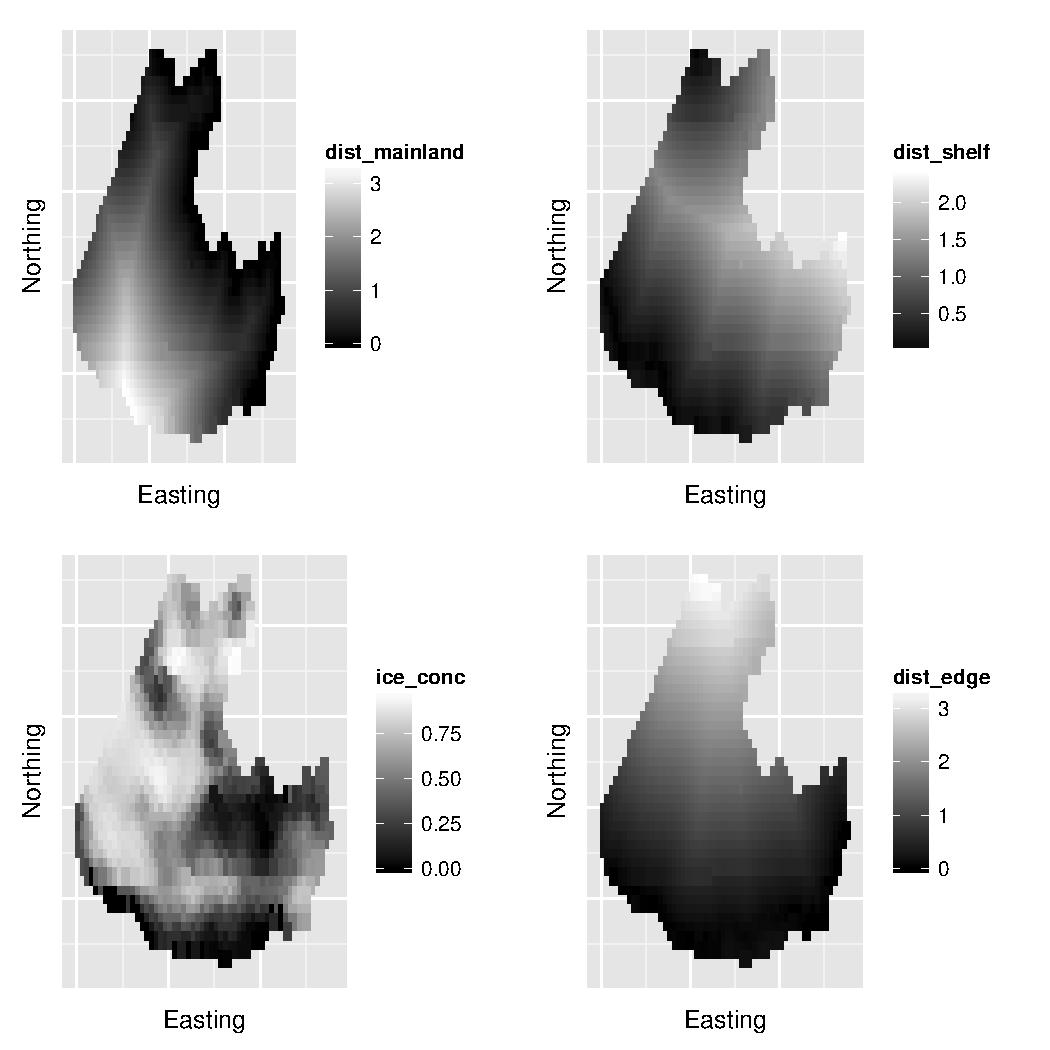
\includegraphics[width=6in]{covariates.pdf}
\end{center}
\caption{ }
\label{fig:covs}
\end{figure}

\begin{figure}[!h]
\begin{center}
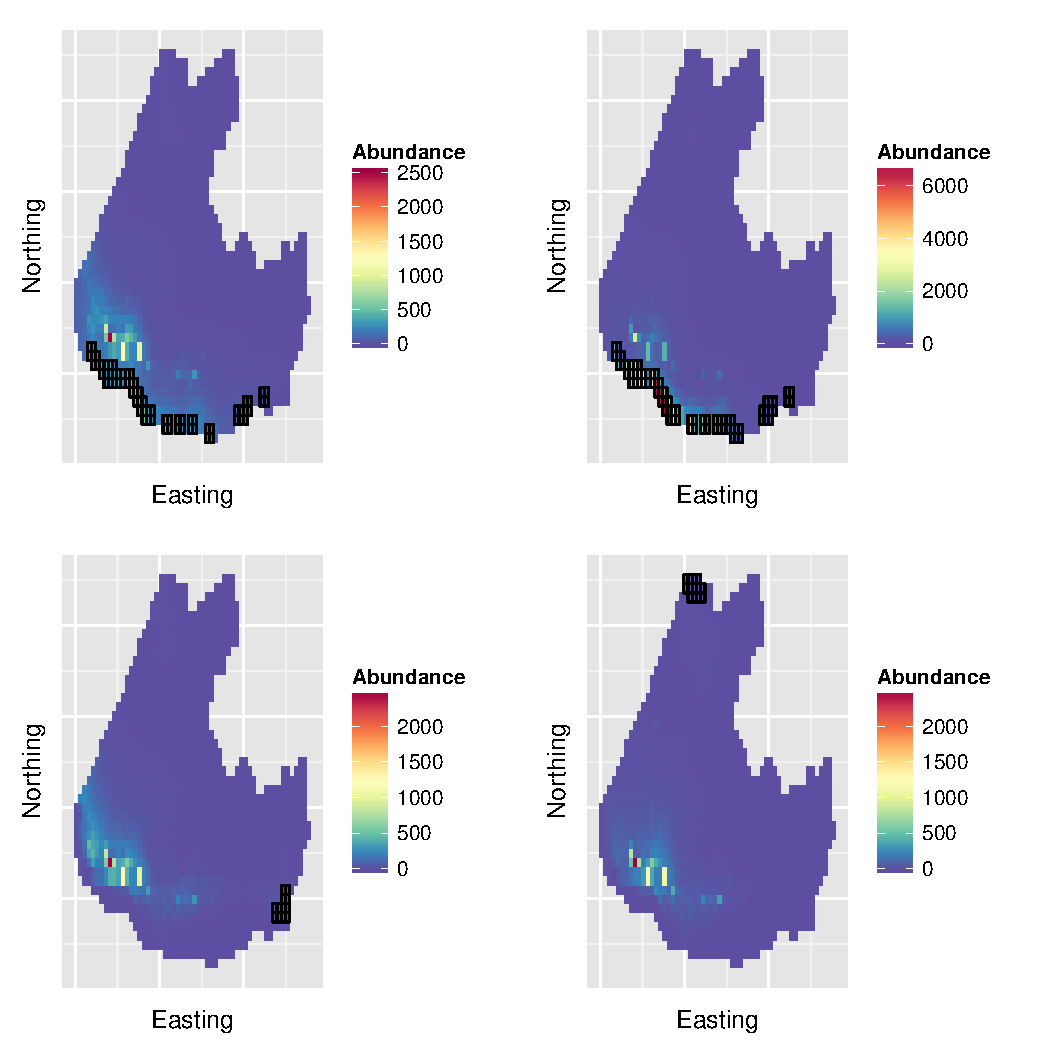
\includegraphics[width=6in]{Bering_noRE_maps.pdf}
\end{center}
\caption{ }
\label{fig:covs}
\end{figure}



\clearpage

\end{spacing}
\end{document} 